% ju 25-Feb-22
\documentclass[11pt,paper=a4,fleqn,parskip=half]{scrartcl}   
\usepackage[T1]{fontenc}            %% Zeichensatzkodierung fuer Silbentrennung
\usepackage[utf8]{inputenc}         %% Unicodezeichen
\usepackage[ngerman]{babel}      %% Dt. Spracheigenschaften
% Schrift
\usepackage{lmodern}
\usepackage[osf,sc]{mathpazo} % Fonts to typeset mathematics to match Palatino
\usepackage{textcase}
\usepackage{nameref}
\usepackage{hyperref}
\usepackage[table,dvipsnames,usenames]{xcolor}%,dvipsnames,usenames, x11names
\usepackage{tabularx}
\usepackage{multirow}
\usepackage{multicol}
\usepackage{caption, booktabs}
\usepackage{graphicx} 
\usepackage{scrhack}    
\usepackage{url}%% Links
\usepackage[inline]{enumitem}
\usepackage{pifont}
\usepackage{eurosym}% \euro 20,-
\usepackage{amsmath}
\usepackage{amsfonts}
\usepackage{amssymb}
\usepackage{array}            % Extending the array and tabular environments
\usepackage{chngcntr}         % Change the resetting of counters
\usepackage[version=4]{mhchem}
\usepackage{stmaryrd}
\usepackage{siunitx}
\usepackage{float}


\parindent0cm %Absatzeinrückung
\usepackage{ragged2e}% Absatzausrichtung: \justifying \Centering \RaggedRight \RaggedLeft
\usepackage{mathtools}
\usepackage{icomma}%Dezimaltrennzeichen
\usepackage{multimedia}%Video: \movie[externalviewer]{(video.mov)}{video.mov}
\usepackage{epstopdf}

\addto\captionsngerman{%
\renewcommand{\figurename}{Abb.}
\renewcommand{\tablename}{Tab.}
}

% eigene Farbe definieren
% Adobe Prozessfarben: CMYK: 100,50,0,35 -> 1,0.5,0,0.35
\definecolor{orange}{cmyk}{0,0.55,0.61,0}   % 0,55,61,0
\definecolor{blau5}{cmyk}{1,0.77,0.1,0.01}  % 100,77,10,
\definecolor{rot5}{cmyk}{0.22,1,1,0.19}   % 22,100,100,19
\definecolor{grau2}{cmyk}{0,0,0,0.1}          % 0,0,0,40
\definecolor{blau}{cmyk}{0.93,0.66,0,0.21}% 


%\usepackage[headsepline,automark]{scrlayer-scrpage} 
% headings
%\pagestyle{scrheadings}
%\automark*[section]{}

\usepackage{latexsym}   % to get the \Box symbol
\usepackage{footnote}
\usepackage{qrcode}% Anwendung: \qrcode[hyperlink,level=Q,version=2,height=1cm]{\website}
\usepackage{underscore}% Unterstrich ____
% PDF Dokumente einbinden
\usepackage{pdfpages}% \includepdf[pages=-]{Tabellen/Inventar-1}

% bibliography
\usepackage[
    bibencoding=utf8,
    backend=biber,% bibtex, biber
    backref=false,backrefstyle=three+,url=true,urldate=comp,abbreviate=false,maxnames=20
]{biblatex} %Paket laden
\DeclareBibliographyCategory{cited}
\let\defaultcite\cite\renewcommand*\cite[2][]{\addtocategory{cited}{#2}\defaultcite[#1]{#2}}
\let\defaulttextcite\textcite\renewcommand*\textcite[2][]{\addtocategory{cited}{#2}\defaulttextcite[#1]{#2}}
\setcounter{biburllcpenalty}{7000}
\setcounter{biburlucpenalty}{8000}
\AfterPackage{biblatex}{
	\PreventPackageFromLoading[\errmessage{Sie haben versucht, das Cite-Paket zu laden, das nicht mit biblatex kompatibel ist.}]{cite}
}


% listings
\usepackage{listings}
\lstset{basicstyle=\linespread{1}\ttfamily\small,floatplacement=!htb,captionpos=t,abovecaptionskip=.5\baselineskip,belowcaptionskip=.5\baselineskip,upquote=true,showstringspaces=false,inputencoding=utf8,tabsize=4,
    	keywordstyle=\bfseries ,
	commentstyle=\color{rot5},
	stringstyle=\color{orange},
	breaklines=true,
  	postbreak=\mbox{\textcolor{black}{$\hookrightarrow$}\space},
	breakatwhitespace=false
}
\lstset{literate={á}{{\'a}}1 {é}{{\'e}}1 {í}{{\'i}}1 {ó}{{\'o}}1 {ú}{{\'u}}1 {Á}{{\'A}}1 {É}{{\'E}}1 {Í}{{\'I}}1 {Ó}{{\'O}}1 {Ú}{{\'U}}1 {à}{{\`a}}1 {è}{{\`e}}1 {ì}{{\`i}}1 {ò}{{\`o}}1 {ù}{{\`u}}1 {À}{{\`A}}1 {È}{{\'E}}1 {Ì}{{\`I}}1 {Ò}{{\`O}}1 {Ù}{{\`U}}1 {ä}{{\"a}}1 {ë}{{\"e}}1 {ï}{{\"i}}1 {ö}{{\"o}}1 {ü}{{\"u}}1 {Ä}{{\"A}}1 {Ë}{{\"E}}1 {Ï}{{\"I}}1 {Ö}{{\"O}}1 {Ü}{{\"U}}1 {â}{{\^a}}1 {ê}{{\^e}}1 {î}{{\^i}}1 {ô}{{\^o}}1 {û}{{\^u}}1 {Â}{{\^A}}1 {Ê}{{\^E}}1 {Î}{{\^I}}1 {Ô}{{\^O}}1 {Û}{{\^U}}1 {œ}{{\oe}}1 {Œ}{{\OE}}1 {æ}{{\ae}}1 {Æ}{{\AE}}1 {ß}{{\ss}}1 {ű}{{\H{u}}}1 {Ű}{{\H{U}}}1 {ő}{{\H{o}}}1 {Ő}{{\H{O}}}1 {ç}{{\c c}}1 {Ç}{{\c C}}1 {ø}{{\o}}1 {å}{{\r a}}1 {Å}{{\r A}}1 {€}{{\EUR}}1 {£}{{\pounds}}1 {~}{{\textasciitilde}}1 {-}{{-}}1 }

\hypersetup{%
	%pdftitle={\titel},
	%pdfsubject={Latex},
	%pdfauthor={\autor},
	%pdfcreator={\autor}, 
	bookmarksnumbered=true,
	breaklinks=true,
	%colorlinks=true,	   
	linkcolor=rot5,		
	filecolor=blau5,		
	urlcolor=blau5,			
	citecolor=ForestGreen
}

%\AtBeginDocument{\recalctypearea}
\linespread{1.1}
\setlist{itemsep=0pt}
\widowpenalty10000
\clubpenalty10000
\tolerance1000    

\usepackage[left=2.0cm,right=2.0cm,top=2.0cm,bottom=2.3cm]{geometry}% quer: landscape
\usepackage{fancyhdr}
\pagestyle{fancy}

%%%%%%%%%%%%%%%%%%%%%%%%%%%%%%%%%%%%%%%%%%%%%
% anpassen
\newcommand{\titel}{\LaTeX}
\newcommand{\name}{Jan Unger}
\newcommand{\datum}{\today}
%\newcommand{\quelle}{\textbf{\copyright \, \name}}% anpassen: (c) oder 
\newcommand{\quelle}{\textbf{Quelle: \, \name}}% anpassen: Quelle:
\newcommand{\logo}{
\includegraphics[height=0.8cm]{images/Logo1.pdf}}% anpassen: Logo oder Datum


\lhead{\quelle}
%\rhead{\logo}
\rhead{}
\title{\titel}

% pro Tabelle: farbige Zeilen im wechsel
%\rowcolors{1}{}{grau2}% EIN / AUS: \showrowcolors o. \hiderowcolors

% Literatur
\bibliography{content/literatur}
\bibliography{content/literatur-kfz}
\bibliography{content/literatur-sport}
\begin{document}
%%%%%%%%%%%%%%%%%%%%%%%%%%%%%%%%%%%%%%%%%%%%%

\begin{center}
	\textbf{\Large \titel}\\%14pt
        \vspace{0.4em}
        \datum
\end{center}

% Zusammenfassung 
\begin{abstract} 
	\textcolor{purple}{>>Zusammenfassung<<}\\
	\vspace{0.4em}
	\raggedleft \small{-- Wikipedia}% 10pt
\end{abstract}

% Check anpassen
\begin{itemize}[label=\checkmark] %\itemsep -2pt
       \item Check
\end{itemize}

    %%%%%%%%%%%%%%%%%%%%%%%%%%%%%%%%%%%%%%%%%%%%%%%%%%%%%%%%%%%%%%%%%%

	% anpassen
	%\input{content/tex/neu}
	%%ju 05-Feb-22 Spickzettel-Markdown.tex
\section{Schreiben in Markdown}\label{schreiben-in-markdown}

\begin{enumerate}
\item
  Markdown
\item
  Textauszeichnung -- Was ist wichtig? Tabellen, Bilder, Quellcode,
  Literatur, Links
\item
  Rechtschreibprüfung \footnote{\url{https://languagetoolplus.com/?pk-campaign=addon2-popup-logo}}
\item
  Literatur \footnote{\url{https://www.zotero.org/user/login}}
\end{enumerate}

\section{Markdown -- Latex -- PDF
erstellen}\label{markdown-latex-pdf-erstellen}

\begin{enumerate}
\item
  Markdown > Latex: \verb|$ projekt.sh|
  Script (pandoc)
\item
  Hand-Kopie: \verb|tex\_pandoc/ tex/|
\item
  Referenzen: Links prüfen

  \begin{itemize}
  \item
    Bild %vgl.~(\autoref{fig:}). >
    \verb|(\\autoref\{fig:bild\}).|
  \item
    Tabelle %vgl.~(\autoref{tab:}). >
    \verb|(\\autoref\{tab:tabellen\}).|
  \item
    Kapitel %vgl.~(\autoref{}). >
    \verb|(\\autoref\{sec:zusammenfassung\}).|
  \item
    Code %vgl.~(\autoref{code:}). >
    \verb|(\\autoref\{code:hallowelt\})|.
  \end{itemize}
\item
  Latex > PDF: \verb|$ make| Makefile
  (latexmk)
\end{enumerate}

\section{Quellen}\label{quellen}

Quelle: \textcite{spanner:2019:robotik}

Quelle: \textcite{homofaciens:2018:projekt}

Quelle: \textcite{kofler:2018:hacking}

\lstset{language=Python}% C, TeX, Bash, Python 
\begin{lstlisting}[
	%caption={}, label={code:}%% anpassen
]
Quelle: [@monk:2016:action]
Quelle: [@homofaciens:2018:projekt]
Quelle: [@kofler:2018:hacking]
\end{lstlisting}

\section{Listen}\label{listen}

\textbf{ungeordnete Liste}

\begin{itemize}
\item
  a
\item
  b

  \begin{itemize}
  \item
    BB
  \end{itemize}
\item
  c
\end{itemize}

\lstset{language=Python}% C, TeX, Bash, Python 
\begin{lstlisting}[
	%caption={}, label={code:}%% anpassen
]
- a
- b
    - bb
- c
\end{lstlisting}

\textbf{Sortierte Liste}

\begin{enumerate}
\item
  eins
\item
  zwei
\item
  drei
\end{enumerate}

\lstset{language=Python}% C, TeX, Bash, Python 
\begin{lstlisting}[
	%caption={}, label={code:}%% anpassen
]
1. eins
2. zwei
3. drei
\end{lstlisting}

\textbf{Sortierte Liste}

\begin{enumerate}
\def\labelenumi{\alph{enumi})}
\item
  a
\item
  b
\item
  c
\end{enumerate}

\lstset{language=Python}% C, TeX, Bash, Python 
\begin{lstlisting}[
	%caption={}, label={code:}%% anpassen
]
a) a
b) b
c) c
\end{lstlisting}

\section{Anführungszeichen}\label{anfuehrungszeichen}

>>Anführungszeichen<<

\lstset{language=Python}% C, TeX, Bash, Python 
\begin{lstlisting}[
	%caption={}, label={code:}%% anpassen
]
"Anführungszeichen" 
\end{lstlisting}

\section{Grafik -- Abbildung}\label{grafik-abbildung}

Logo %vgl.~(\autoref{fig:}).

\begin{figure}[!ht]% hier: !ht
\centering

\includegraphics[width=0.3\textwidth]{images/Logo/logo.pdf}
\caption{Logo}
%\label{fig:}%% anpassen
\end{figure}

\lstset{language=Python}% C, TeX, Bash, Python 
\begin{lstlisting}[
	%caption={}, label={code:}%% anpassen
]
![Logo](images/Logo/logo.pdf){width=30%}
\end{lstlisting}

\section{Tabelle}\label{tabelle}

Tabelle-Bsp %vgl.~(\autoref{tab:}).

\begin{table}[!ht]% hier: !ht 
\centering 
	\caption{}% \label{tab:}%% anpassen 
\begin{tabular}{@{}rll@{}}
\hline
\textbf{Nr.} & \textbf{Begriffe} & \textbf{Erklärung} \\
\hline
1 & a1 & a2 \\
2 & b1 & b2 \\
3 & c1 & c2 \\
4 & a1 & a2 \\
\hline
\end{tabular} 
\end{table}

\lstset{language=Python}% C, TeX, Bash, Python 
\begin{lstlisting}[
	%caption={}, label={code:}%% anpassen
]
| **Nr.** | **Begriffe** | **Erklärung** |
| --: | :----- | :---- |
|       1 | a1           | a2            |
|       2 | b1           | b2            |
|       3 | c1           | c2            |
|       4 | a1           | a2            |
\end{lstlisting}

\section{Mathematik}\label{mathematik}

$[ V ] = [ \Omega ] \cdot [ A ]$ o. $U = R \cdot I$ o.
$R = \frac{U}{I}$

\lstset{language=Python}% C, TeX, Bash, Python 
\begin{lstlisting}[
	%caption={}, label={code:}%% anpassen
]
$[ V ] = [ \Omega ] \cdot [ A ]$ o. $U = R \cdot I$ o. $R = \frac{U}{I}$
\end{lstlisting}

$5~cm$, $a \cdot b$, $\cdots$, $\Omega$

$100^\circ\text{C}$

$80~\%$ // in HTML

\lstset{language=Python}% C, TeX, Bash, Python 
\begin{lstlisting}[
	%caption={}, label={code:}%% anpassen
]
$5~cm$, $a \cdot b$, $\cdots$, $\Omega$
$100^\circ\text{C}$  
// ACHTUNG: Prozentzeichen macht Probleme in HTML und Latex 
// Z.B. 80 %
$80~\%$ // in Latex
$80~\%$  // in HTML
\end{lstlisting}

\textbf{Mathematik-Umgebung:}

\begin{align*}
    \sum_{i=1}^5 a_i = a_1 + a_2 + a_3 + a_4 + a_5
\end{align*}

\lstset{language=Python}% C, TeX, Bash, Python 
\begin{lstlisting}[
	%caption={}, label={code:}%% anpassen
]
\begin{align*}
    \sum_{i=1}^5 a_i = a_1 + a_2 + a_3 + a_4 + a_5
\end{align*}
\end{lstlisting}

\section{Texthervorhebung}\label{texthervorhebung}

\textbf{Fett} oder \emph{Kursiv}

\lstset{language=Python}% C, TeX, Bash, Python 
\begin{lstlisting}[
	%caption={}, label={code:}%% anpassen
]
**Fett** oder *Kursiv*
\end{lstlisting}

\section{Code}\label{code}

Hallo Welt %vgl.~(\autoref{code:}).

\lstset{language=Python}% C, TeX, Bash, Python 
\begin{lstlisting}[
	%caption={}, label={code:}%% anpassen
]
// hallowelt.c
#include <stdio.h>
int main(void) {
    printf("Hallo Welt!\n");
    return 0;
}
\end{lstlisting}

\section{Links}\label{links}

\url{https://google.de} oder \href{https://google.de}{Google}

\lstset{language=Python}% C, TeX, Bash, Python 
\begin{lstlisting}[
	%caption={}, label={code:}%% anpassen
]
<https://google.de> oder [Google](https://google.de)
\end{lstlisting}

Fußnote\footnote{\url{https://bw-ju.de/}}

\lstset{language=Python}% C, TeX, Bash, Python 
\begin{lstlisting}[
	%caption={}, label={code:}%% anpassen
]
Fußnote[^1]       

[^1]: <https://bw-ju.de/>
\end{lstlisting}

\section{Absätze}\label{absaetze}

Dies hier ist ein Blindtext zum Testen von Textausgaben. Wer diesen Text
liest, ist selbst schuld. Der Text gibt lediglich den Grauwert der
Schrift an. Ist das wirklich so? Ist es gleichgültig, ob ich schreibe:
>>Dies ist ein Blindtext<< oder >>Huardest gefburn<<? Kjift -
mitnichten! Ein Blindtext bietet mir wichtige Informationen. An ihm
messe ich die Lesbarkeit einer Schrift, ihre Anmutung, wie harmonisch
die Figuren zueinander stehen und prüfe, wie breit oder schmal sie
läuft. Ein Blindtext sollte möglichst viele verschiedene Buchstaben
enthalten und in der Originalsprache gesetzt sein. Er muss keinen Sinn
ergeben, sollte aber lesbar sein.

Fremdsprachige Texte wie >>Lorem ipsum<< dienen nicht dem eigentlichen
Zweck, da sie eine falsche Anmutung vermitteln.
 
 	%%Inhalt
\section*{Hallo} Jetzt geht's los...

\textbf{fetter Text} \footnote{Text}


Quelle \footnote{\textcite{kofler:2018:hacking}}.

\section{Welche Zeichen dürfen verwendet werden?}

Ziffern: 0…9
Buchstaben: a…z A…Z\\
Sonderzeichen:  . : ; , ? ! ( ) [ ] + - * / = @\\
Steuerzeichen: \$ \& \% \# \_ \{ \} \textasciitilde \textasciicircum \textbackslash \textbar \\
Umlaute: ä ö ü ß Ä Ö Ü\\
Anführungszeichen: "`Hallo!"' ``Hello!'' "<Salut!">\\
Gedankenstrich: - -- \\
EURO-Symbol: \euro

\section{Abstand}

Text

\smallskip etwa $\frac{1}{4}$ Zeile Abstand

\medskip etwa $\frac{1}{2}$ Zeile Abstand

\bigskip etwa $1$ Zeile Abstand

\vspace{2ex} %Relative Maßangabe: für Höhen

Abstand durch vspace

Text \hspace{2em} Abstand durch hspace%Relative Maßangabe:  für Breiten

Abstand durch Leerzeile

\section{Farbe}

\textcolor{red}{Text} \colorbox{red}{\textcolor{white}{Text}}
\textcolor{blau}{Text} \colorbox{blau}{\textcolor{white}{Text}}
\textcolor{orange}{Text} \colorbox{orange}{\textcolor{white}{Text}}
\textcolor{gray}{Text} \colorbox{gray}{\textcolor{white}{Text}}
\textcolor{purple}{Text} \colorbox{purple}{\textcolor{white}{Text}}

\section{Code}

\begin{lstlisting}[language={[LaTeX]TeX}]
% HalloWelt.tex
\documentclass{article}
\begin{document}
	Hallo Welt!
\end{document}
\end{lstlisting}

\begin{lstlisting}[language={C}]
// HalloWelt.c
#include <stdio.h>
int main(void){
	printf("Hallo Welt!\n");
	return 0;
}
\end{lstlisting}

\section*{Mathe}
 
 $x^{2} + px + q = 0$

\begin{equation}
 x_{1,2} = -\frac{p}{2} \pm \sqrt{D}
\end{equation}
 
\begin{align*}
(a+b)^{2}  &= (a+b) (a+b) \\
                &= a^{2} + ab + ba + b^{2} \\
                &= a^{2} + 2ab + b^{2}
\end{align*}

Dezimaltrennzeichen: $1,23$ $1.23$

Exponenten, Indizes, Vektor: $x_{1} \,  x^{2} \, \vec{x}$

\begin{equation}
x = y^{-1} \text{ für alle $y > 0$ }
\end{equation}

Griechische Buchstaben: $\alpha \, \Omega$

Mathematische Symbole: $\le \, \sim \, \ne \, \approx \, \notin$

$\ldots \, \cdots \, \{ \, \} \rightarrow \, \left( \frac{x+a}{x-a} \right)^2$

Brüche, Wurzeln, Binomialkoeffizienten, Summen, Grenzwerte

$\frac{1}{2} \, \frac{x^2}{x^2+1} \, \sqrt{x} \, \sqrt[4]{x^2+1} \, \binom{n}{k} \, \sin x \, \sum\limits_{i=1}^{n} i \, \lim\limits_{x \to 0}$

Matrizen und Fallunterscheidungen

$\boldsymbol{A} = \left(
	\begin{matrix} 
		1 & 2 & 3 \\
		4 & 5 & 6 \\
		7 & 8 & 9
	\end{matrix} 
\right)$

$
f(x) =
\begin{cases}
	   -x  & \text{f"ur $x < 0$} \\
	    1  & \text{f"ur $x = 0$} \\
	\ln x  & \text{f"ur $x > 0$}
\end{cases}
$

$\boxed{E=mc^2}$




\section{Boxen}

\fbox{Text}

\fbox{Text Text \raisebox{-1.0ex}{ Text nach unten } \raisebox{1.0ex}{ Text nach oben } Text Text}

\fbox{
\begin{tabular}{cp{5cm}}
$A \cap B$ &
$A$ und $B$ treten gleichzeitig ein.\\
$A \cup B$ &
Es tritt $A$ oder es tritt $B$ ein
(beide zugleich sind möglich).
\end{tabular}
}

 \section{Bild}
 
 \fbox{

\includegraphics[height=6cm,angle=30]{images/Logo/Logo1.pdf}

\includegraphics[height=4cm,angle=-30]{images/Logo/Logo2.pdf}
 }


Bild (\autoref{fig:bild}).
\begin{figure}[!h]% hier: !hb
	\centering
	
\includegraphics[width=.55\textwidth]{images/Logo/logo.eps}
	\caption{Bild}\label{fig:bild}%% anpassen
\end{figure}
 
 
 \section{Links}
 
 PDF öffnen: (\url{images/Logo/Logo-Details.pdf}) 
 
 Video öffnen: \movie[externalviewer]{(video.mov)}{images/Video/video.mov}
 
 Website \footnote{\url{http://bw-ju.de/}}

\section{Tabelle}

% Tab 1
(siehe \autoref{tab:heisetabelle}).
\begin{table}[ht]
\centering
\begin{tabular}{cc}
\toprule 
\textbf{Begriff} & \textbf{Definition}\\
\midrule  
A	&	Text \\
B	&	Text \\ 
C	&	Text \\
D	&	Text \\
E	&	Text \\
F	&	Text \\
\bottomrule
\end{tabular}
\caption{Beschreibung der Tabelle}
\label{tab:heisetabelle}
\end{table}


% Tab 2
\rowcolors{1}{}{grau2}% EIN: oder \showrowcolors o. \hiderowcolors
\begin{table}[h]
\centering
\begin{tabular}{cp{3.5cm}}
\textbf{Begriff} & \textbf{Definition}\\
\hline %\showrowcolors %\hiderowcolors
A	&	Text \\
B	&	Text \\ 
C	&	Text \\
D	&	Text \\
E	&	Text \\
F	&	Mehrzeiliger Text \newline in einer Zelle \\
\end{tabular}
\caption{Beschreibung}
\label{tab:tabelle}
\end{table}
\rowcolors{1}{}{}% AUS

%\newpage
%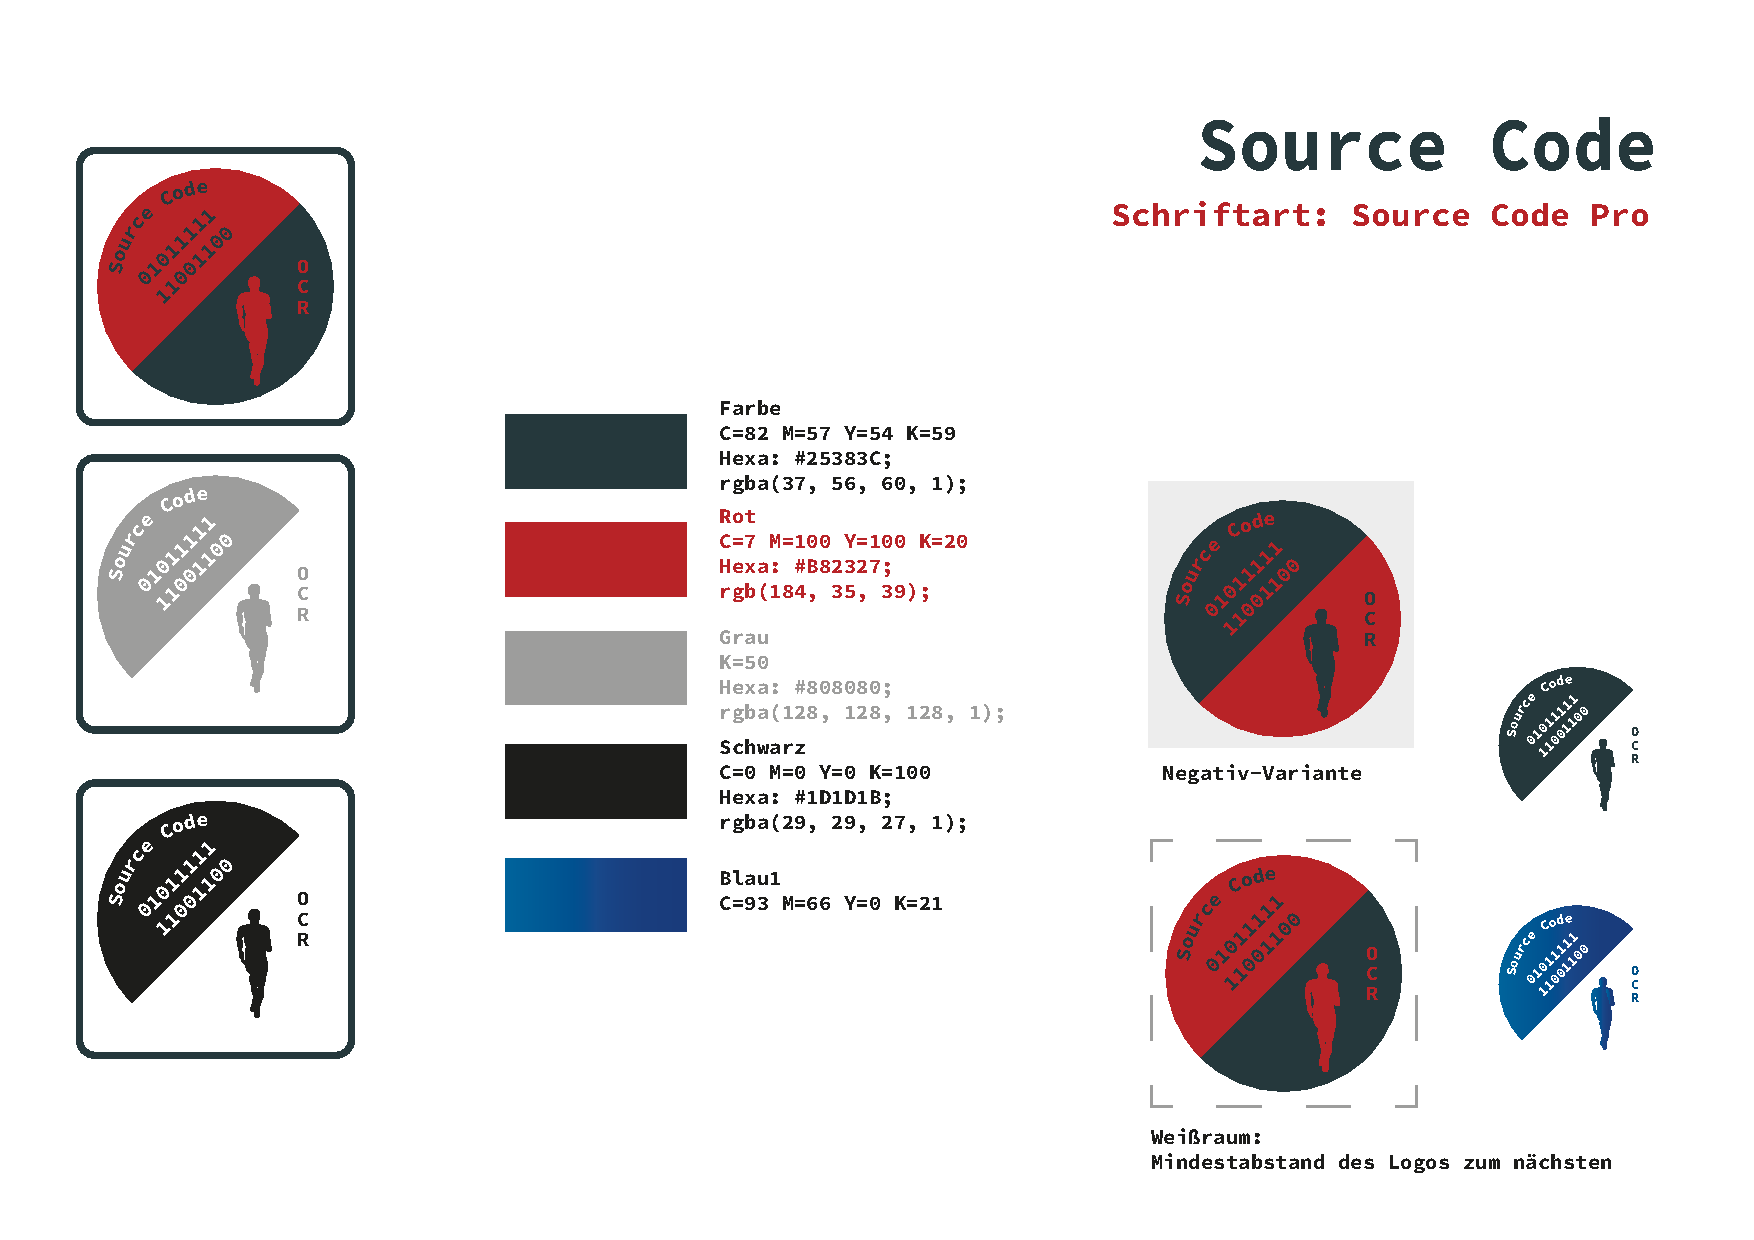
\includepdf[pages=-,landscape]{images/Logo/Logo-Details.pdf}%landscape
 
    %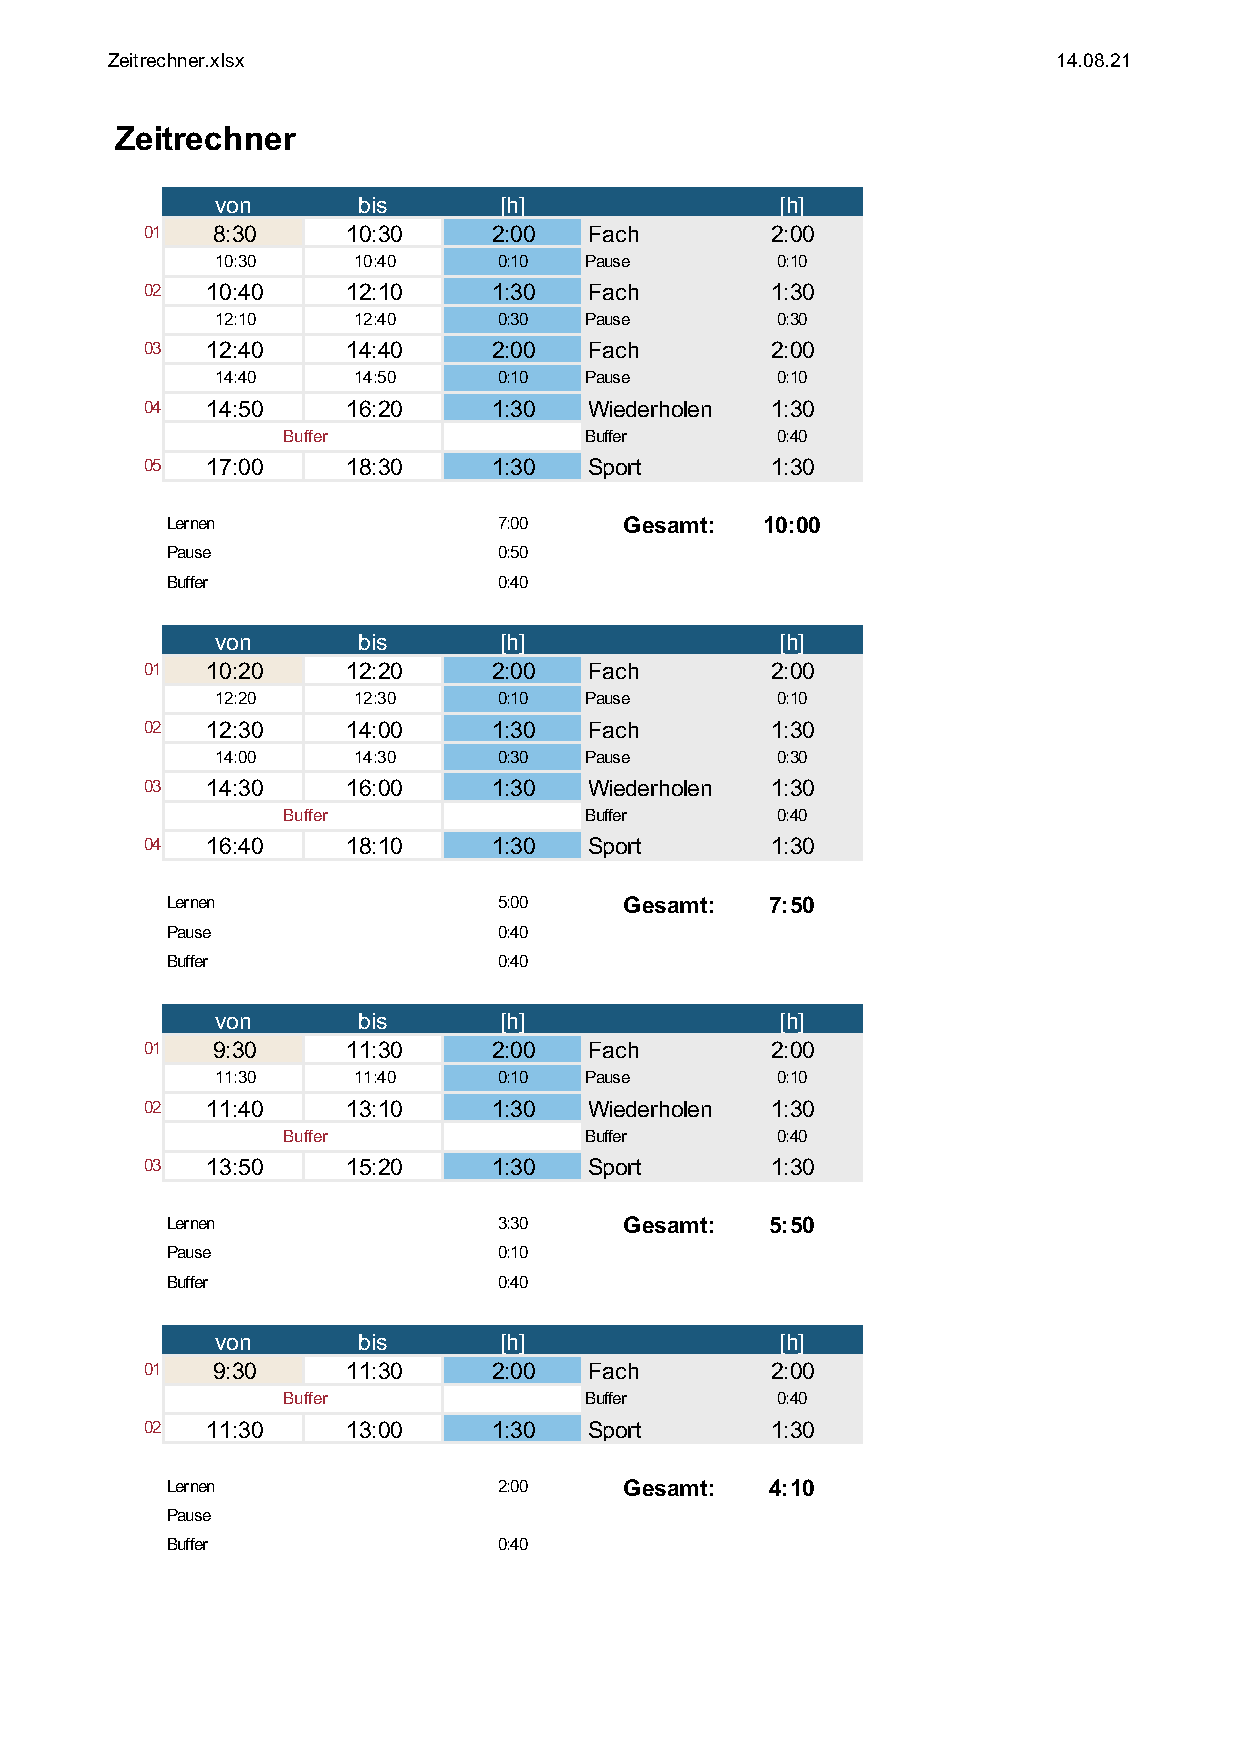
\includepdf[pages=-]{Tabellen/PDF/Zeitrechner.pdf}
	% ju 23-Jul-21
\section*{Einleitung}

\emph{Sonderzeichen}  wie <<\& oder \%>> müssen mit einem Backslash \verb|\& oder \%| maskiert werden, 
damit sie von LaTeX nicht als Befehle missverstanden werden.


\emph{Website} \footnote{\url{https://golatex.de/wiki/Hauptseite}} \verb|\footnote{\url{https://golatex.de/wiki/Hauptseite}}| 


\clearpage
\subsection*{Stand der Forschung}

Während die traditionelle Latexproduktion bereits hinreichend erforscht ist (\autoref{fig:latex}) \\
\verb|(\autoref{fig:latex})|, bleibt das wissenschaftliche Verständnis elektronischer Verarbeitungsprozesse dieses 
vielseitigen Materials weiterhin lückenhaft. 


\begin{figure}[!ht]% hier: !ht
	\centering
	
\includegraphics[width=0.25\textwidth]{images/Logo/logo.eps}
	\caption{Traditionelle Latexproduktion}\label{fig:latex}%
\end{figure}

\clearpage
\section*{Ausblick}

Daraus ergeben sich gemäß (\autoref{tab:schritte}) \verb|(\autoref{tab:schritte})| folgende nächste Schritte, 
deren sequenzielle Ausführung von essenzieller Bedeutung ist.

\begin{table}[!ht]% hier: !ht
	\centering
	\begin{tabular}{@{}cl@{}}% lcr
		\toprule
		\textbf{Nr.} & \textbf{Vorgehen} \\
		\midrule
		1 & Aktuellen Forschungsstand recherchieren \\
		2 & Methoden entwickeln \\
		3 & Schlussfolgerung aufstellen \\
		\bottomrule
	\end{tabular}
	\caption{Nächste Schritte}\label{tab:schritte}
\end{table}



	%%%%%%%%%%%%%%%%%%%%%%%%%%%%%%%%%%%%%%%%%%%%%%%%%%%%%%%%%%%%%%%%%%
    % Bibliographie
    %\printbibliography
\end{document}
